%%%%%%%%%%%%%%%%%%%%%%%%%%%%%%%%%%%%%%%%%
%
% Paritition Presentation
% LaTeX 
% Version 1.0 (08/12/14)
%
%%%%%%%%%%%%%%%%%%%%%%%%%%%%%%%%%%%%%%%%%

%----------------------------------------------------------------------------------------
% PACKAGES AND THEMES
%----------------------------------------------------------------------------------------

\documentclass{beamer}

\mode {
\usetheme{Madrid}
}

\usepackage{graphicx} % Permite introducir imagenes
\usepackage{booktabs} % Allows the use of \toprule, \midrule and \bottomrule in tables
\usepackage{amsfonts} % Simbolos
\usepackage{amssymb} % Simbolos
\usepackage{amsmath} % matematicos
\usepackage{graphicx} % imagenes

%----------------------------------------------------------------------------------------
% TITLE PAGE
%----------------------------------------------------------------------------------------

% Titulo de la presentacion
\title[ PARTITION ]{ Partition }

% Autores
\author{Sawan J. Kapai Harpalani \and
Adri\'an Gonz\'alez Mart\'in \and
Sara Mart\'in Molina \and
Enrique Tejera Gonz\'alez
}

% Institucion a la que pertenecen los colaboradores
\institute[ULL] 
{
Universidad de La Laguna \ 
\medskip
}

% Fecha de hoy
\date{\today}

% Comienzo del documento
\begin{document}

\begin{frame}

% Imprime el titulo
\titlepage

\end{frame}

%----------------------------------------------------------------------------------------
% DIAPOSITIVAS DE LA PRESENTACION
%----------------------------------------------------------------------------------------

\begin{frame}
\frametitle{Partition}
% Comenzamos una enumeracion
\begin{itemize}
\item Teorema: Partition es NP-Completo.
\item Instancia: A, a $\in$ A y S(a) $\in$ (\mathbb{Z})$\textsuperscript{+}$.
\item Prueba: Es f\'acil ver que partition $\in$ NP, puesto que es un algoritmo
no determinista necesita s\'olo encontrar un subconjunto A' de A y comprobar el
tiempo polinomial que suma los tama~{n}os de los elementos de A' es igual a la
suma de los elementos de A - A'.

\end{itemize}

\end{frame}

%------------------------------------------------

\begin{frame}
\frametitle{Transformaci\'on 3DM a Partition}
\begin{itemize}
\item Se fijan los conjuntos W, X, Y con tama~{n}o q y M que ser\'a una instancia
arbitraria del 3DM (M $\subseteq$ $W \times X \times Y$).
$$W = w_{1}, w_{2}, w_{3}, \ldots w_{q}$$
$$X = x_{1}, x_{2}, x_{3}, \ldots x_{q}$$
$$Y = y_{1}, y_{2}, y_{3}, \ldots y_{q}$$
$$M = m_{1}, m_{2}, m_{3}, \ldots m_{k}$$ 
$$ k = |M|$$

\item Se debe construir un conjunto A, donde cada elemento tiene tama~{n}o tal que S(a) $\in$ (\mathbb{Z})$\textsuperscript{+}$ y ese A debe contener un subconjunto A' tal que:
$$\sum\limits_{a \in A'} S(a) = \sum\limits_{a \in A - A'} S(a) \iff si \ M \ contiene \ Matching$$
\item El conjunto A contendr\'a k + 2 elementos.
\end{itemize}
\end{frame}

%------------------------------------------------

\begin{frame}
\frametitle{Construcci\'on}
El conjunto A se construye en dos pasos:
\begin{enumerate}
\item Primer paso:
\begin{itemize}
\item Los primeros k elementos de A est\'an asociados con las k tripletas de M
$$ a_{i} \Rightarrow m_{i}, 1 \leq i \leq k $$
\item El tama~{n}o de cada elemento se obtiene de su representaci\'on binaria. Esta representaci\'on contendr\'a q zonas con p bits cada una.
$$ |W| = |X| = |Y| = q $$
$$p = [\log_2(k + 1)]$$
\end{itemize}

\end{enumerate}

\end{frame}

%------------------------------------------------

\begin{frame}
\frametitle{Construcci\'on}
\begin{enumerate}
\item Primer paso:
\begin{itemize}
\item La representaci\'on binaria del elemento $a_{i}$ depende de la tripleta:
$$m_{i} = (w_{f(i)}, x_{g(i)}, y_{h(i)}) \in M$$
\item Otra forma de obtener el tama~{n}o de $a_{i}$:
$$S(a_{i}) = 2\textsuperscript{p(3q - f(i))} + 2\textsuperscript{p(2q - g(i))} + 2\textsuperscript{p(q - h(i))}$$
\end{itemize}

\end{enumerate}

\end{frame}

%------------------------------------------------

\begin{frame}
\frametitle{Construcci\'on}
\begin{enumerate}
\item Primer paso:
\begin{itemize}
\item Si se fija:
$$B = \sum\limits_{j=0}^{3q -1} 2\textsuperscript{pj}$$
\item Entonces:
$$A'\subseteq {a_{i}: 1 \leq i \leq k}$$
$$\sum\limits_{a\in A'} = B \iff M' = {m_{i}: a_{i} \in A' \Rightarrow matching(M)}$$
\end{itemize}

\end{enumerate}

\end{frame}

%------------------------------------------------

\begin{frame}
\frametitle{Construcci\'on}
\begin{enumerate}
\setcounter{enumi}{1}
\item Segundo paso:
\begin{itemize}
\item Se especifican los dos \'ultimos elementos de A ($b_{1}$ y $b_{2}$) cuyos tama~{n}os son:
$$S(b_{1}) = 2(\sum\limits_{i=1}^{k}S(a_{i})) - B $$
$$S(b_{2}) = (\sum\limits_{i=1}^{k}S(a_{i})) + B $$
\item Ambos pueden ser especificados en binario con no m\'as de (3pq + 1) bits.
\end{itemize}

\end{enumerate}

\end{frame}

%------------------------------------------------

\begin{frame}
\frametitle{Construcci\'on}
\begin{enumerate}
\setcounter{enumi}{1}
\item Segundo paso:
\begin{itemize}
\item Suponiendo que se tiene un conjunto $A' \subseteq A$ se cumple:
$$\sum\limits_{a \in A'} S(a) = \sum\limits_{a \in A - A'} S(a)$$
\item Por lo que las sumas de ambos ser\'a:
$$ 2\sum\limits_{i=1}^{k}S(a_{i})$$
\item Uno de los conjuntos, $A'\ o \ A - $A', contendr\'a $b_{1}$ pero no $b_{2}$.
\end{itemize}

\end{enumerate}

\end{frame}

%------------------------------------------------

\begin{frame}
\frametitle{Construcci\'on}
\begin{enumerate}
\setcounter{enumi}{1}
\item Segundo paso:
\begin{itemize}
\item El resto de elementos formar\'an un subconjunto de:
$$a_{i}: 1 \leq i \leq k$$
\item La suma de los tama~{n}os de esos elementos es igual a B, por lo que ese subconjunto es un matching de M' en M.
\item A la inversa, si tenemos un matching M':
$${b_{1} \bigcup {a_{1}}: m_{i} \in M' \ forma \ A' \ para \ la \ instancia \ de \ Partition } $$
\item Por lo tanto 3DM se puede transformar en Partition en tiempo polinomial
\end{itemize}

\end{enumerate}

\end{frame}

%------------------------------------------------

\begin{frame}
\frametitle{Ejemplo}
\begin{figure}[ht!]
\centering
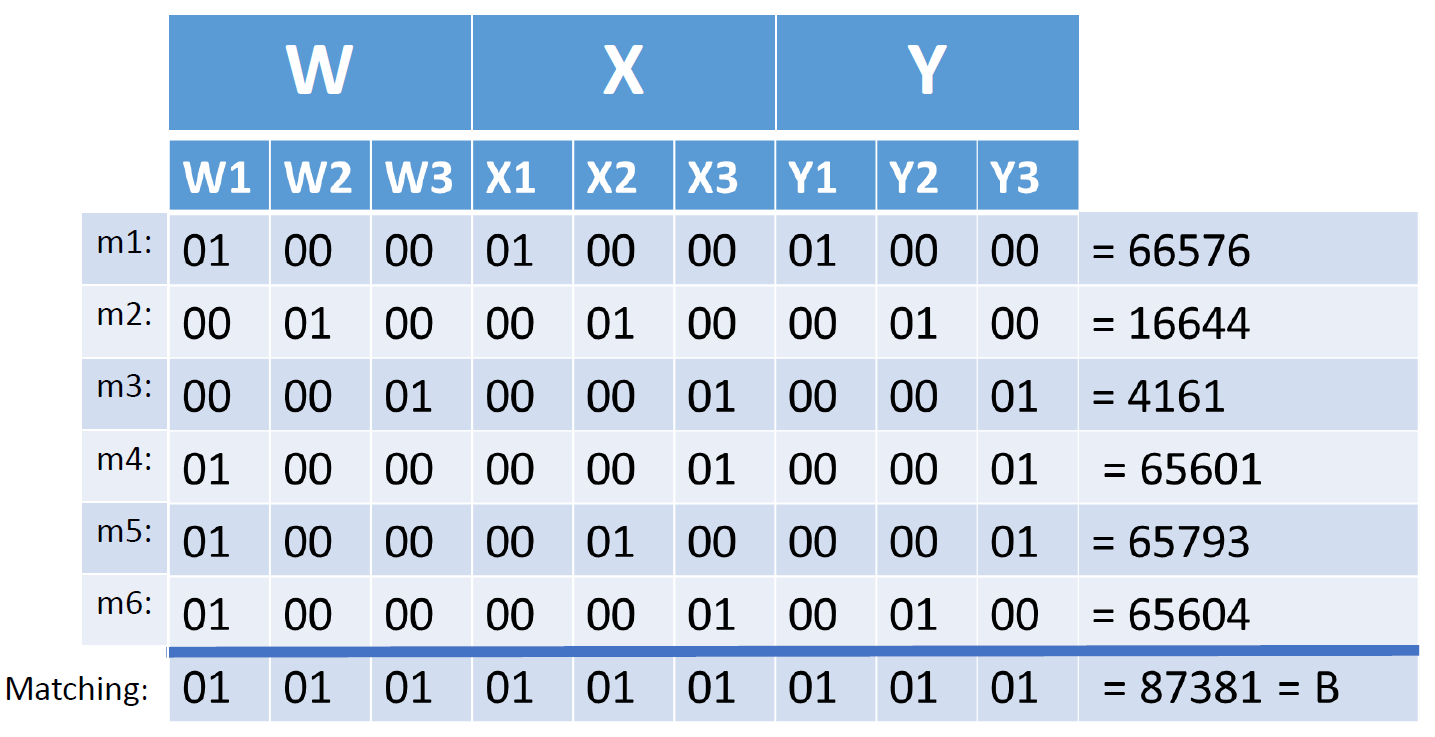
\includegraphics[width=90mm]{images/partition.png}
\caption{Ejemplo \label{overflow}}
\end{figure}
\end{frame}

%------------------------------------------------

\begin{frame}
\Huge{\centerline{FIN}}
\end{frame}

%----------------------------------------------------------------------------------------

\end{document}